
\documentclass{article}

\usepackage{fullpage}
\usepackage{amsmath}
\usepackage{amscd}
\usepackage[tableposition=top]{caption}
\usepackage{ifthen}
\usepackage[utf8]{inputenc}
\usepackage[pdftex]{graphicx}
\usepackage{placeins}

\usepackage{Sweave}
\begin{document}

\title{Assignment 3}
\author{Christopher Peters}
\maketitle

\section{Assignment 3: Exercise 1}

The file Bleed.txt, in RSplidaAlpha\textbackslash RSplida text data, contains
field failure data on failures in aircraft engine bleed systems (each air-
craft has one such system) from a fleet of 2256 military aircraft. Use
these data to compute the Kaplan-Meier product limit estimator out to
500 hours of operation. Set this up in a table and do the computation
without the aid of a computer, unless you do your own programming
(e.g., in R or an Excel spreadsheet). Show the table outlining the com-
putations as part of your solution. You can use available software (e.g.
JMP or RSPLIDA) to check your answers.\\


{\bf Answer:}





\begin{figure}[htbp]
\begin{center}
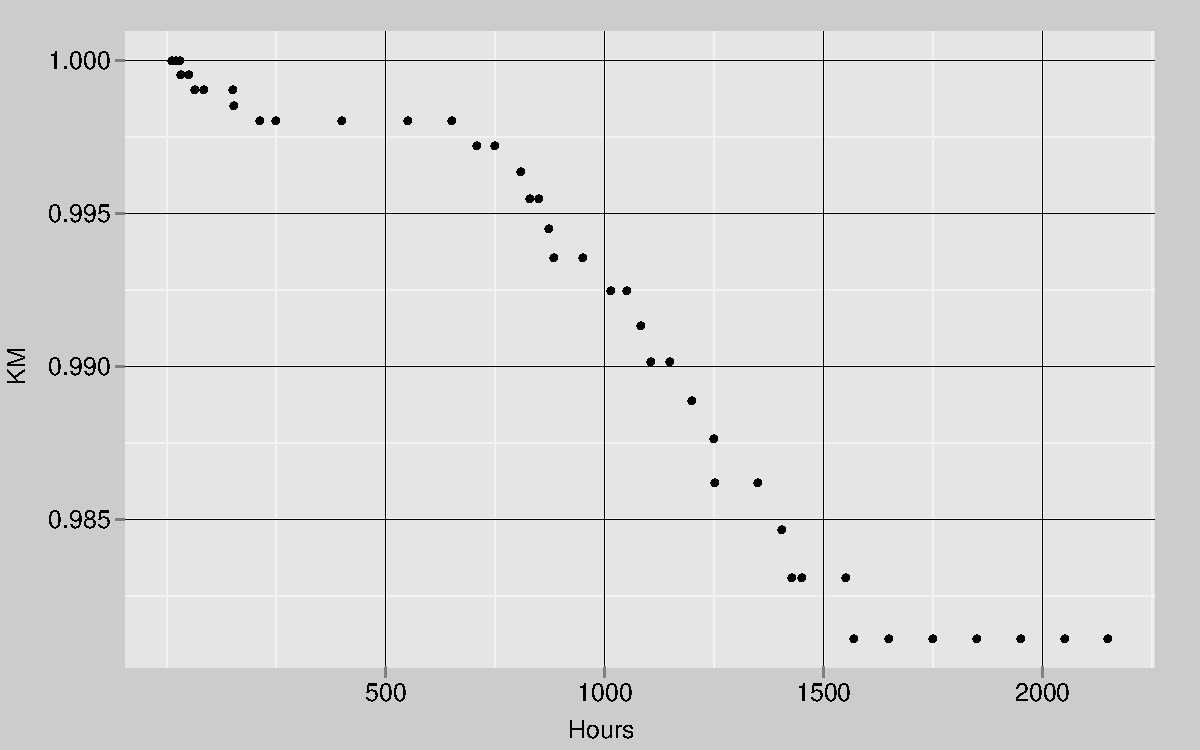
\includegraphics{assignment3_sweave_2-004}
\caption{Figure 1: Kaplan-Meier Estimates}
\end{center}  
\end{figure}

\begin{center}
% latex table generated in R 2.13.1 by xtable 1.6-0 package
% Sat Dec 03 16:13:22 2011
\begin{table}[ht]
\begin{center}
\begin{tabular}{rrlrrrrr}
  \hline
 & Hours & Status & Weight & units.entered & d & pi & KM \\ 
  \hline
1 & 12 & Censored & 39 & 2256 & 0 & 1.00000000 & 1.00000000 \\ 
  2 & 20 & Censored & 52 & 2217 & 0 & 1.00000000 & 1.00000000 \\ 
  3 & 30 & Censored & 46 & 2165 & 0 & 1.00000000 & 1.00000000 \\ 
  4 & 32 & Failed & 1 & 2119 & 1 & 0.99952808 & 0.99952808 \\ 
  5 & 50 & Censored & 31 & 2118 & 0 & 1.00000000 & 0.99952808 \\ 
  6 & 64 & Failed & 1 & 2087 & 1 & 0.99952084 & 0.99904915 \\ 
  7 & 85 & Censored & 48 & 2086 & 0 & 1.00000000 & 0.99904915 \\ 
  8 & 150 & Censored & 102 & 2038 & 0 & 1.00000000 & 0.99904915 \\ 
  9 & 153 & Failed & 1 & 1936 & 1 & 0.99948347 & 0.99853311 \\ 
  10 & 212 & Failed & 1 & 1935 & 1 & 0.99948320 & 0.99801707 \\ 
  NA &  &  &  &  &  &  &  \\ 
  50 & 1650 & Censored & 55 & 490 & 0 & 1.00000000 & 0.98108263 \\ 
  51 & 1650 & Censored & 8 & 435 & 0 & 1.00000000 & 0.98108263 \\ 
  52 & 1750 & Censored & 55 & 427 & 0 & 1.00000000 & 0.98108263 \\ 
  53 & 1750 & Censored & 4 & 372 & 0 & 1.00000000 & 0.98108263 \\ 
  54 & 1850 & Censored & 55 & 368 & 0 & 1.00000000 & 0.98108263 \\ 
  55 & 1850 & Censored & 2 & 313 & 0 & 1.00000000 & 0.98108263 \\ 
  56 & 1950 & Censored & 152 & 311 & 0 & 1.00000000 & 0.98108263 \\ 
  57 & 1950 & Censored & 3 & 159 & 0 & 1.00000000 & 0.98108263 \\ 
  58 & 2050 & Censored & 152 & 156 & 0 & 1.00000000 & 0.98108263 \\ 
  59 & 2050 & Censored & 3 & 4 & 0 & 1.00000000 & 0.98108263 \\ 
  60 & 2150 & Censored & 1 & 1 & 0 & 1.00000000 & 0.98108263 \\ 
   \hline
\end{tabular}
\caption{Kaplan-Meier Computations}
\label{tab:one}
\end{center}
\end{table}\end{center}
\FloatBarrier

\section{Assignment 3: Exercise 3}

The natural logarithm of a Weibull random variable has a smallest extreme value distribution.  Starting with the Weibull distribution in the traditional parametrization (\(\eta \) and \(\beta \)), show this.  Note that this can be done in terms of the cdf or the pdf.  Try to do it both ways.\\

Starting with a Weibull CDF:\\

\begin{Large}
  \begin{align}
      1 - exp[(-\frac{x}{\eta})^{\beta}]\\
      \text{But we're given:} \hspace{.25 cm} 
                            \beta = \frac{1}{\sigma} 
                              \hspace{.25 cm}  \text{and} \hspace{.25 cm}
                             \eta = exp(\mu)\\
      1 - exp\Bigl[-\Bigl(\frac{exp(x)}{exp(\mu)}\Bigr)^{\frac{1}{\sigma}}\Bigr]\\
      1 - exp\Bigl[-exp\Bigl(\frac{x - \mu}{\sigma})\Bigr]\\
      1 - exp\Bigl[-exp\Bigl(\frac{x - \mu)}{\sigma}\Bigr)\Bigr] \longrightarrow \Phi_{SEV}
  \end{align}
\end{Large}




\end{document}
